\documentclass[10pt, xcolor = svgnames]{beamer} %Beamer
\usepackage{palatino} %font type
\usefonttheme{metropolis} %Type of slides
\usefonttheme[onlymath]{serif} %font type Mathematical expressions
\usetheme[progressbar = frametitle,titleformat frame=smallcaps,numbering=counter]{metropolis} %This adds a bar at the beginning of each section.
\useoutertheme[subsection=false]{miniframes} %Circles in the top of each frame, showing the slide of each section you are at

\usepackage{appendixnumberbeamer} %enumerate each slide without counting the appendix
\setbeamercolor{progress bar}{fg=Maroon!70!Coral} %These are the colours of the progress bar. Notice that the names used are the svgnames
\setbeamercolor{title separator}{fg=DarkSalmon} %This is the line colour in the title slide
\setbeamercolor{structure}{fg=black} %Colour of the text of structure, numbers, items, blah. Not the big text.
\setbeamercolor{normal text}{fg=black!87} %Colour of normal text
\setbeamercolor{alerted text}{fg=DarkRed!60!Gainsboro} %Color of the alert box
\setbeamercolor{example text}{fg=Maroon!70!Coral} %Colour of the Example block text


\setbeamercolor{palette primary}{bg=NavyBlue!50!DarkOliveGreen, fg=white} %These are the colours of the background. Being this the main combination and so one. 
\setbeamercolor{palette secondary}{bg=NavyBlue!50!DarkOliveGreen, fg=white}
\setbeamercolor{palette tertiary}{bg=NavyBlue!40!Black, fg= white}
\setbeamercolor{section in toc}{fg=NavyBlue!40!Black} %Color of the text in the table of contents (toc)

%These next packages are the useful for Physics in general, you can add the extras here. 
\usepackage{amsmath, amssymb}
\usepackage{slashed}
\usepackage{cite}
\usepackage{relsize}
\usepackage{caption}
\usepackage{subcaption}
\usepackage{multicol}
\usepackage{booktabs}
\usepackage[scale=2]{ccicons}
\usepackage{pgfplots}
\usepgfplotslibrary{dateplot}
\usepackage{geometry}
\usepackage{xspace}
\newcommand{\themename}{\textbf{\textsc{bluetemp}\xspace}}%metropolis}}\xspace}

\title{SpectrogramCNN Model}
\author[Name]{Gauss Chang \inst{$\dagger$} and supervisor's name \inst{$\ddagger$}} %With inst, you can change the institution they belong
\subtitle{Training Report}



%\institute[uni]{\inst{\dagger} Department of Physics \\ \textsc{National Taiwan University} \\ \inst{\ddagger} Department of Something \\ \textsc{Supervisor's Institute}}


\institute[uni] % (optional)
{
  \inst{\dagger}%
  Department of Physics \\
  \textsc{National Taiwan University}
  \and
  \inst{\ddagger}%
  Department of Something \\
  \textsc{Supervisor's Institute}
}



\date{\today} %Here you can change the date
\titlegraphic{\vspace{0.0cm}\hfill
\includegraphics[width = 0.25\textwidth]{logo.pdf}}

\begin{document}
{
\setbeamercolor{background canvas}{bg=NavyBlue!50!DarkOliveGreen, fg=white}
\setbeamercolor{normal text}{fg=white}
\maketitle
}%This is the colour of the first slide. bg= background and fg=foreground

\metroset{titleformat frame=smallcaps} %This changes the titles for small caps

\begin{frame}{Outline}
  \setbeamertemplate{section in toc}[sections numbered] %This is numbering the sections
  \tableofcontents[hideallsubsections] %You can comment this line if you want to show the subsections in the table of contents
\end{frame}


\section{About Model}



%\begin{frame}[fragile]{About Model: Structure}
%\tiny
%{
%\begin{verbatim}
%Number of parameter: 42072258.00
%[INFO] Register count_convNd() for <class 'torch.nn.modules.conv.Conv2d'>.
%[INFO] Register count_normalization() for <class 'torch.nn.modules.batchnorm.BatchNorm2d'>.
%[INFO] Register zero_ops() for <class 'torch.nn.modules.pooling.MaxPool2d'>.
%[INFO] Register zero_ops() for <class 'torch.nn.modules.dropout.Dropout'>.
%[INFO] Register count_linear() for <class 'torch.nn.modules.linear.Linear'>.
%The model has 648152576.0 FLOPs
%\end{verbatim}
%}
%\end{frame}

\begin{frame}[fragile]{About Model: Structure}
\tiny
{
\begin{verbatim}
torch.Size([1, 2])
Number of parameters: 42072258.00
[INFO] Register count_convNd() for <class 'torch.nn.modules.conv.Conv2d'>.
[INFO] Register count_normalization() for <class 'torch.nn.modules.batchnorm.BatchNorm2d'>.
[INFO] Register zero_ops() for <class 'torch.nn.modules.pooling.MaxPool2d'>.
[INFO] Register zero_ops() for <class 'torch.nn.modules.dropout.Dropout'>.
[INFO] Register count_linear() for <class 'torch.nn.modules.linear.Linear'>.
The model has 648152576.0 FLOPs
\end{verbatim}
}
\end{frame}



\begin{frame}[fragile]{About Model: Structure}
\begin{figure}
\centering
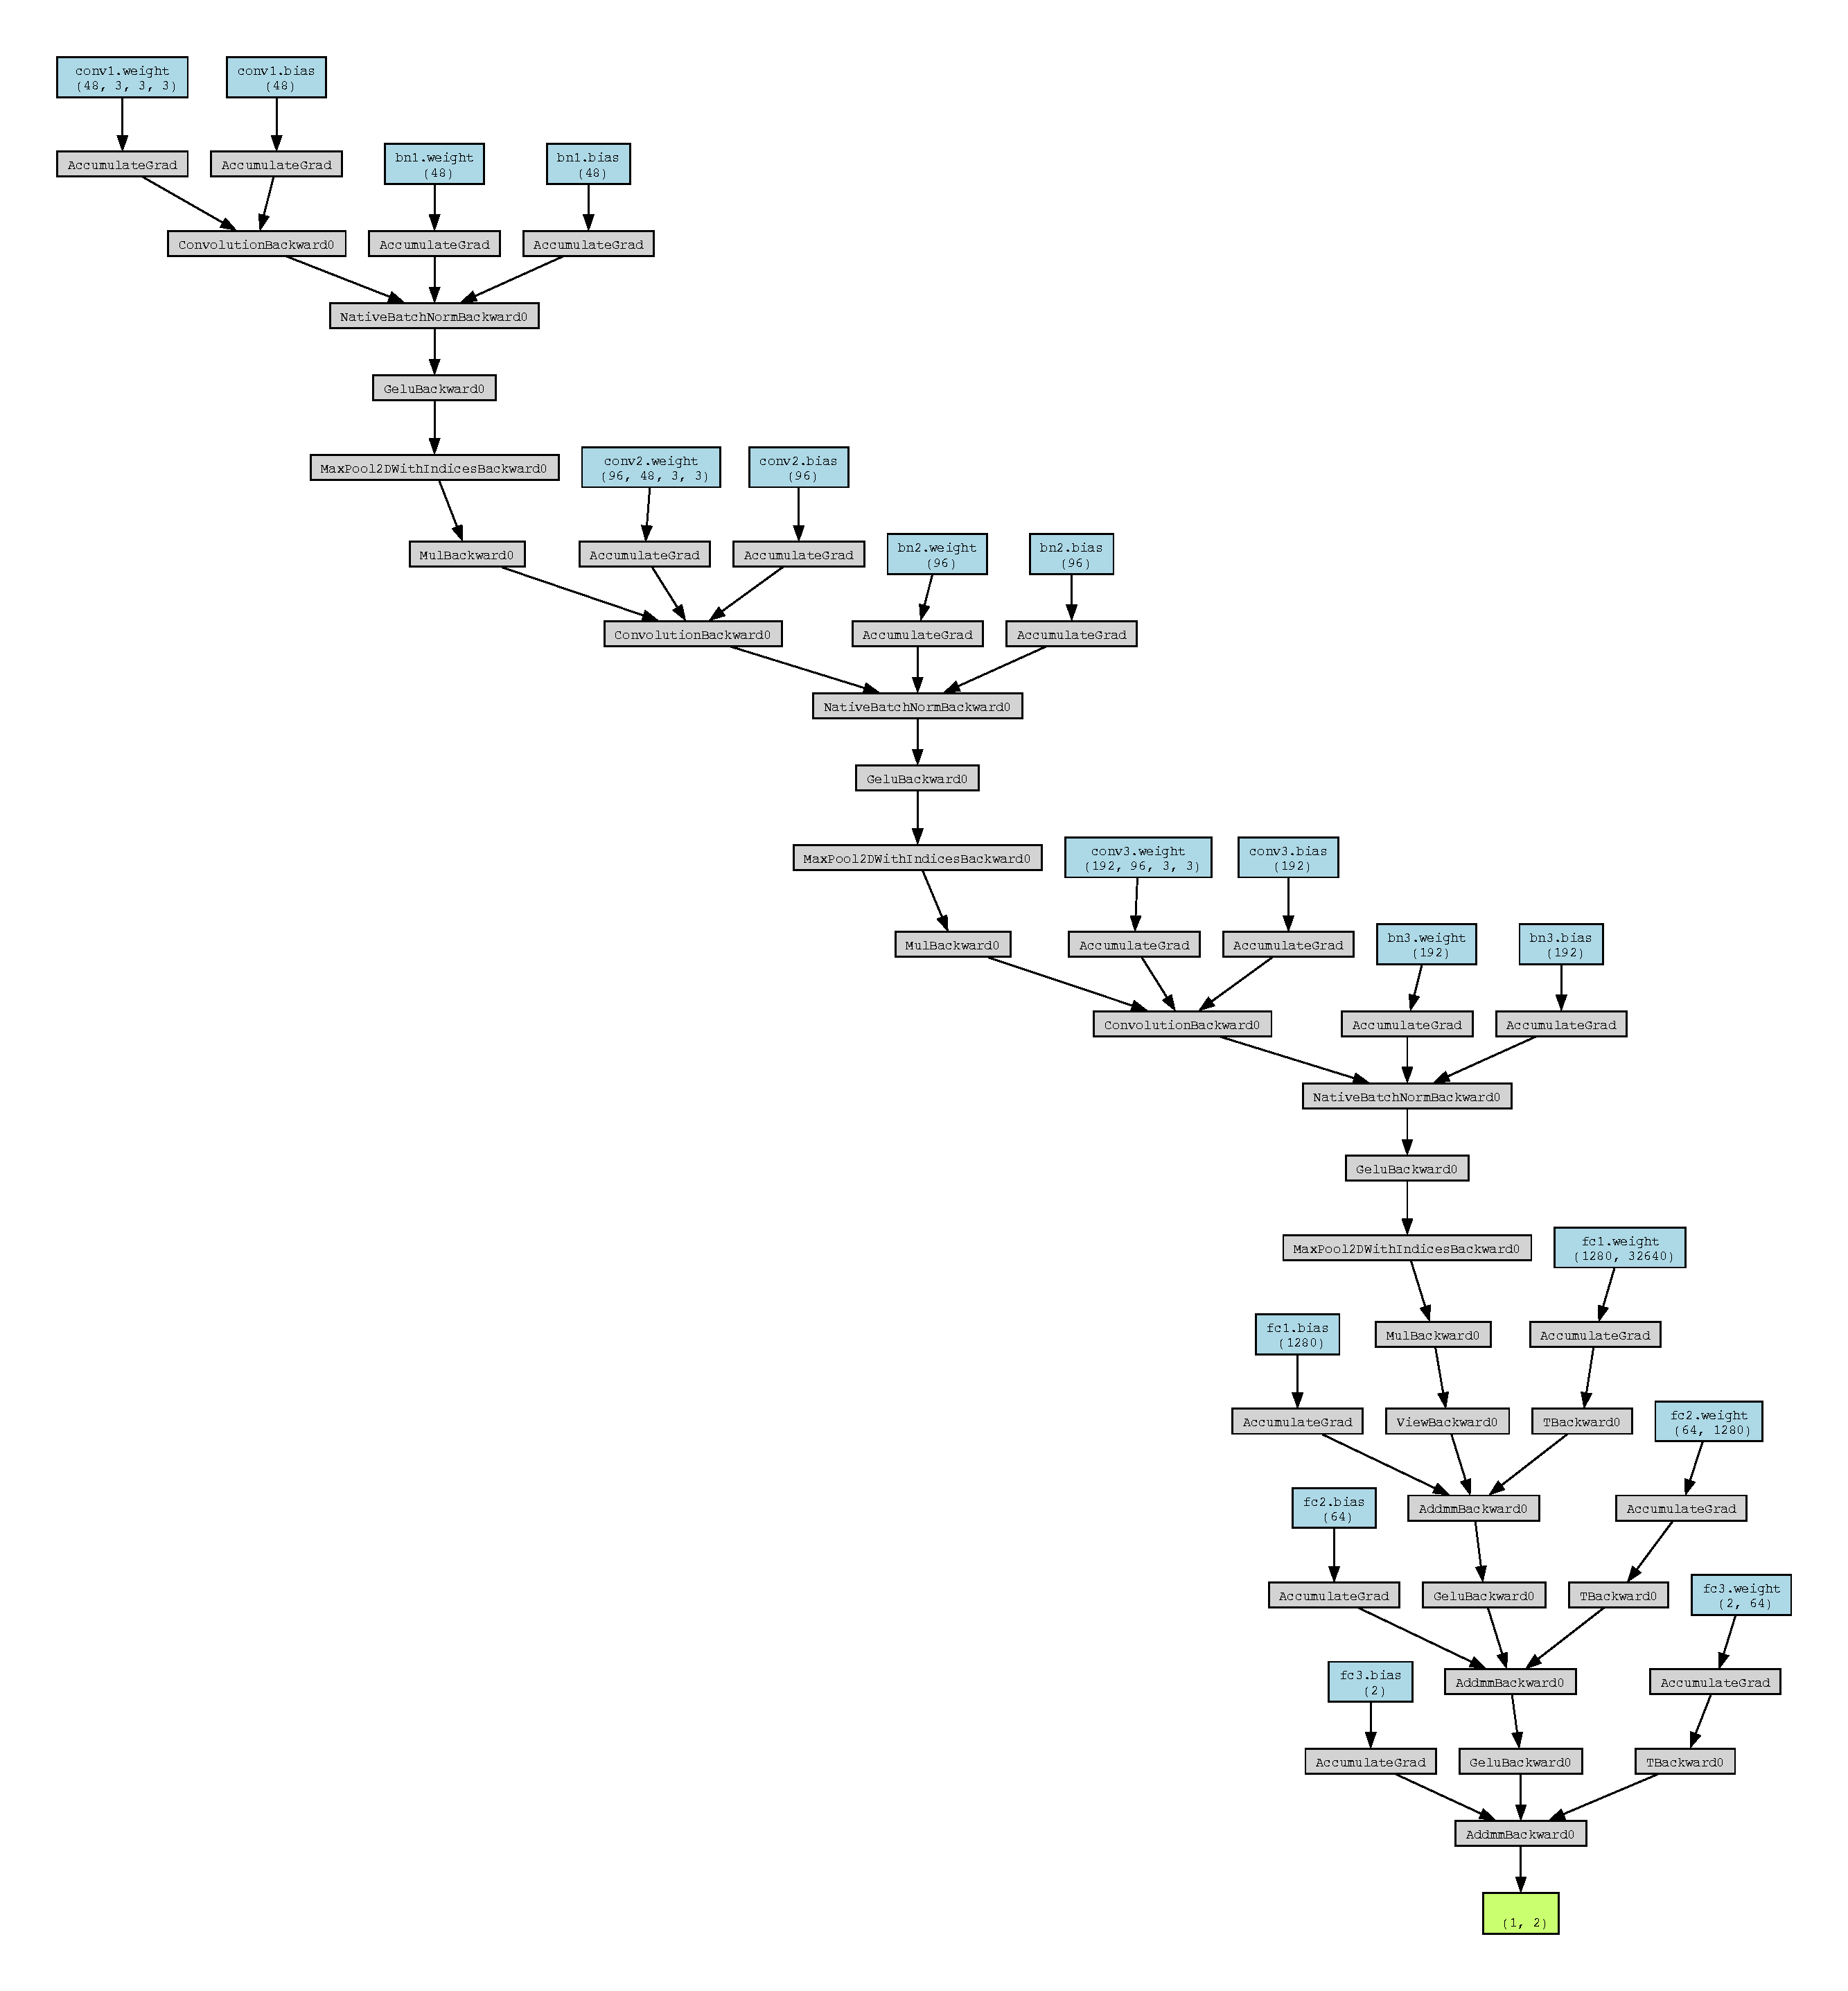
\includegraphics[width = 0.65\textwidth]{../model_structure/SpectrogramCNN_Model.pdf}
\label{fig1}
\end{figure}
\end{frame}



\section{Accuracy}



\begin{frame}[fragile]{Accuracy: Confusion Matrix}
\begin{figure}
\centering
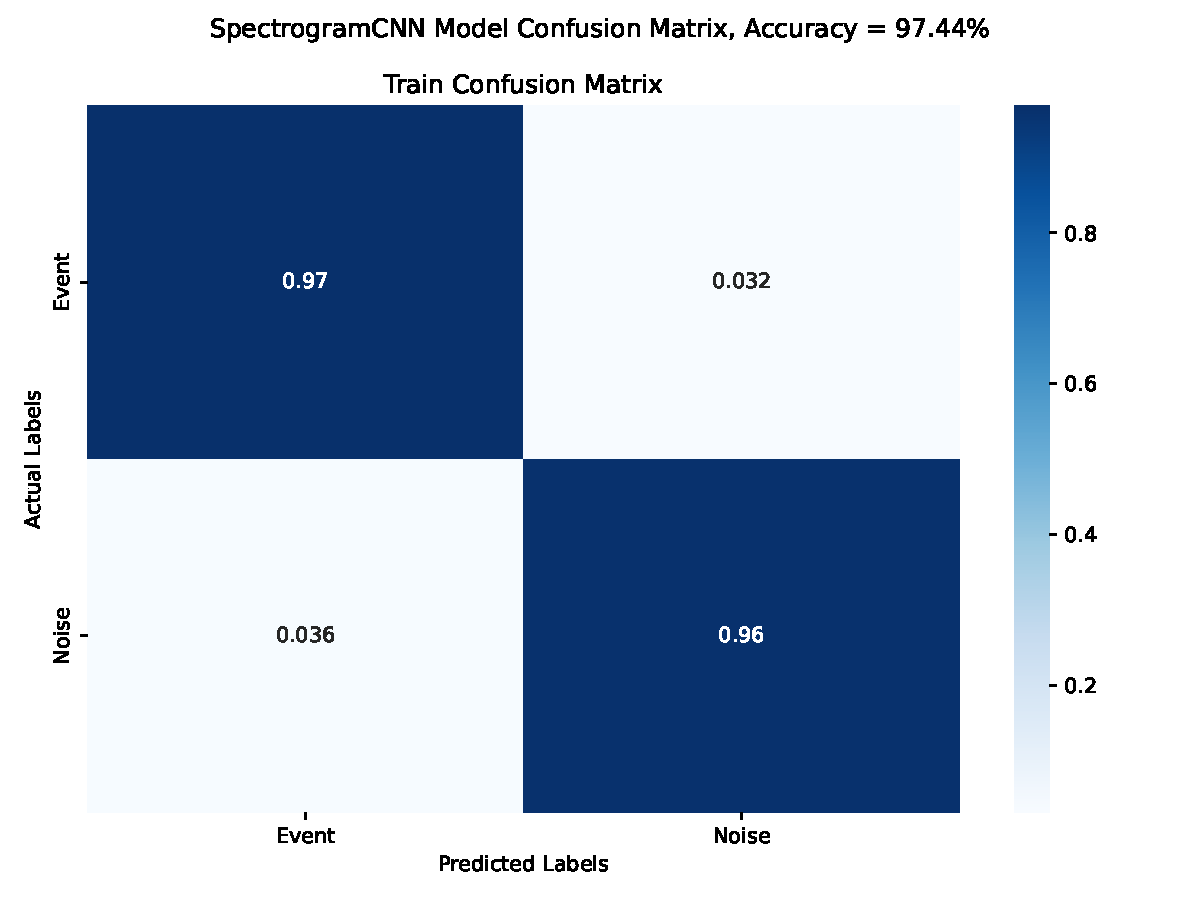
\includegraphics[width = 0.8\textwidth]{../Spectrogram_Result/Spectrogram_CM.pdf}
\label{fig1}
\end{figure}
\end{frame}


\begin{frame}[fragile]{Accuracy: Accuracy Curve}
\begin{figure}
\centering
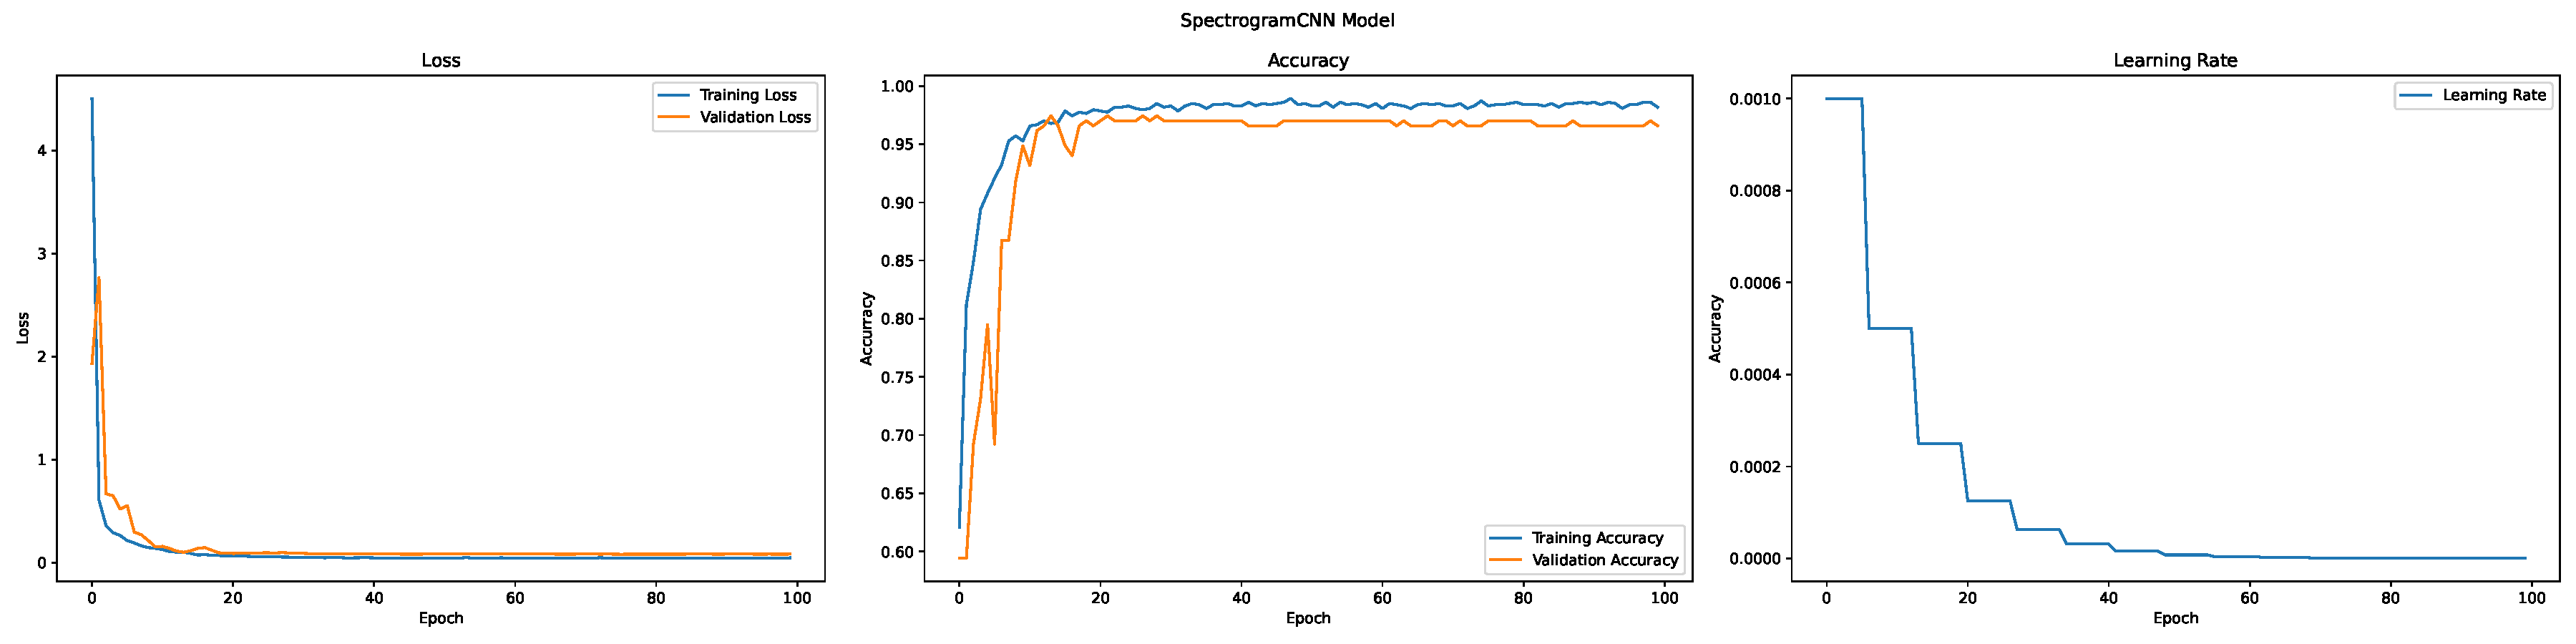
\includegraphics[width = 1.0\textwidth]{../Spectrogram_Result/Spectrogram_Accurracy.pdf}
\label{fig1}
\end{figure}
\end{frame}



\section{Time Evaluation}

\begin{frame}[fragile]{Time Evaluation: On Linux PC}
\tiny
{
\begin{verbatim}If execute on the Linux PC, check here
================================================================================
Maximum time on Mac mini is:       69.976000 ms.
Average time on Mac mini is:       12.582552 ms.
Standard dev on Mac mini is:        3.194686 ms.
--------------------------------------------------------------------------------
Maximum time on Raspberry Pi 4b should be:      538.276923 ms.
Average time on Raspberry Pi 4b should be:       96.788859 ms.
Standard dev on Raspberry Pi 4b should be:        8.860465 ms.
================================================================================
\end{verbatim}
}
\end{frame}

\begin{frame}[fragile]{Time Evaluation: On Mac mini}
\tiny
{
\begin{verbatim}If execute on the Mac mini, check here
================================================================================
Maximum time on Mac mini is:       69.976000 ms.
Average time on Mac mini is:       12.582552 ms.
Standard dev on Mac mini is:        3.194686 ms.
--------------------------------------------------------------------------------
Maximum time on Raspberry Pi 4b should be:      496.283688 ms.
Average time on Raspberry Pi 4b should be:       89.237955 ms.
Standard dev on Raspberry Pi 4b should be:        8.507826 ms.
================================================================================
\end{verbatim}
}
\end{frame}

\begin{frame}[fragile]{Time Evaluation: On Macbook 2017}
\tiny
{
\begin{verbatim}If execute on the Macbook 2017, check here
================================================================================
Maximum time on Mac mini is:       69.976000 ms.
Average time on Mac mini is:       12.582552 ms.
Standard dev on Mac mini is:        3.194686 ms.
--------------------------------------------------------------------------------
Maximum time on Raspberry Pi 4b should be:      171.826346 ms.
Average time on Raspberry Pi 4b should be:       30.896506 ms.
Standard dev on Raspberry Pi 4b should be:        5.006088 ms.
================================================================================
\end{verbatim}
}
\end{frame}


\end{document}












